\documentclass[10pt,twocolumn]{article}

\usepackage[margin=0.75in,columnsep=0.3in]{geometry}
\usepackage{times}
\usepackage{amsmath}
\usepackage{graphicx}
\usepackage{booktabs}
\usepackage{natbib}
\usepackage{hyperref}
\usepackage{xcolor}
\usepackage{caption}
\usepackage[T1]{fontenc}

\setlength{\parskip}{0.25em}
\setlength{\parindent}{0pt}
\captionsetup{font=small}

\hypersetup{
  colorlinks=true,
  linkcolor=blue,
  citecolor=blue,
  urlcolor=blue,
}

\title{\vspace{-2em}Length-Dependent Quantization Fragility in Audio State Space Models}
\author{Ayush Urs \\ \small University of California San Diego \\ \small \texttt{aurs@ucsd.edu}}
\date{}

\begin{document}

\twocolumn[
\begin{@twocolumnfalse}
\maketitle
\begin{abstract}
\small
Selective state space models (SSMs) such as Mamba compress an entire sequence into a fixed-size recurrent state, updated at every step, while attention gives every token direct, uncompressed access to every other token. We ask whether this compression makes SSM-based audio encoders more fragile to post-training quantization than Transformer-based ones, and if so, which internal tensor is responsible. Using two official, task-matched checkpoints on Speech Commands V2 (Audio Mamba, AuM, and the Audio Spectrogram Transformer, AST), we find that standard Linear-layer quantization does \emph{not} explain AuM's fragility: AuM's accuracy already collapses to near-chance from full precision alone, immediately past its $\sim$1s training length, leaving quantization nothing additional to degrade by top-1 accuracy. AST degrades far more gradually with length and shows a real, bit-width-specific W4A16 accuracy drop at 40--80s. We then isolate AuM's own internal SSM tensors ($\Delta$, $A$, $B/C$, and the recurrent state $h$) one at a time at native length, where AuM still has accuracy headroom. A nonparametric bootstrap over 140 class-balanced clips shows the recurrent state is fragile from the mildest bit-width tested (83.6\% at 8-bit, falling to 7.9\% at 4-bit), $\Delta$ holds up through 6-bit (88.6\%) before collapsing between 6- and 4-bit (19.3\%), while $A$ and $B/C$ remain within noise of full precision at every bit-width tested (95--97\%). Per-timestep state-divergence traces show these two failure shapes are qualitatively different: the state's error accumulates smoothly every step, while $\Delta$'s is heavy-tailed, with most steps barely perturbed and a minority blowing up. Code, data manifests, and all raw results are public.\footnote{\url{https://github.com/ayush11z/audio-ssm-quant}}
\end{abstract}
\vspace{1em}
\end{@twocolumnfalse}
]

\section{Introduction}

Selective SSMs \citep{gu2023mamba} process a sequence with linear time and memory complexity by compressing all past context into a fixed-size recurrent state $h_t$, updated at every step as $h_t = \bar{A}_t h_{t-1} + \bar{B}_t x_t$ with $\bar{A}_t = \exp(\Delta_t A)$. This is structurally different from self-attention, which keeps every token's representation and lets any token attend to any other directly, with no compression bottleneck. Audio Mamba (AuM) \citep{erol2024aum} applies this architecture to spectrogram classification as a direct, bidirectional analogue of the Audio Spectrogram Transformer (AST) \citep{gong2021ast}, making the two models an unusually clean pair for isolating the effect of the SSM's compressed-state design from everything else (patch embedding, classification head, training data).

Post-training quantization (PTQ) adds a second source of approximation error on top of a model's own architecture. We ask two questions. \textbf{H1:} does PTQ hurt AuM more than AST, and does that gap widen as input length grows past AuM's $\sim$1-second training length, where the state has to summarize far more than it was trained to? \textbf{H2:} if the SSM's internals are a distinct source of fragility, which specific tensor in the recurrence -- $\Delta$, the state-transition parameter $A$, the input/output projections $B,C$, or the recurrent state $h$ itself -- actually drives it?

We find H1 is the wrong frame for top-1 accuracy: AuM's full-precision accuracy already collapses to near-chance immediately past its training length (\S\ref{sec:h1}), leaving no headroom for quantization to measurably remove. AST, which degrades far more gradually, shows the only clear quantization-specific accuracy effect in the whole grid. For H2, a tensor-isolated ablation at native length (\S\ref{sec:h2}) finds two of AuM's four internal tensors genuinely fragile, with different failure shapes, while the other two are essentially quantization-proof.

\section{Related Work}

\textbf{Models.} Mamba \citep{gu2023mamba} introduced input-dependent (``selective'') SSM parameters as a linear-time alternative to attention. AuM \citep{erol2024aum} is the first purely SSM-based audio classifier, built as a bidirectional counterpart to AST \citep{gong2021ast}; both have official checkpoints fine-tuned on Speech Commands V2 \citep{warden2018speechcommands}, used directly here, with no retraining.

\textbf{Quantization.} General PTQ for large Transformers (e.g.\ GPTQ \citep{frantar2023gptq}) targets Linear weights almost exclusively, since attention has no persistent numerical state to protect. Two recent works, MambaQuant \citep{xu2025mambaquant} and Quamba2 \citep{chiang2025quamba2}, build PTQ \emph{recipes} specifically for the Mamba family and both independently flag the selective-scan's activations/state as the hard part to quantize -- Quamba2 reports ``massive outliers'' in the scan's output activations and applies a dedicated per-state-group scheme to $B,C$ to control them. We differ in kind, not just scale: rather than a deployable quantizer, we run a controlled ablation isolating \emph{which single tensor} is responsible, as a function of input length, which these recipe papers do not study. Our finding that the state $h$ is the most fragile tensor, with $\Delta$ fragile only past a bit-width threshold and $B,C$ robust under plain per-tensor quantization, is consistent with Quamba2's choice to specially protect the scan's state/activations, and gives a tensor-level account of why.

\section{Method}

\textbf{Models.} AuM-Base (bidirectional, \texttt{bimamba\_v1}, 24 layers, embed dim 768, AudioSet-pretrained then fine-tuned on Speech Commands V2) and AST (\texttt{MIT/ast-finetuned-speech-commands-v2}) -- both official checkpoints for the identical 35-class task, avoiding a cross-dataset confound. $128\times128$-mel-bin log-spectrograms, $16\times16$ patches.

\textbf{Data.} Speech Commands V2 \citep{warden2018speechcommands}, 35 keyword classes. Native clips are $\sim$1s (both checkpoints' training length). Length-extended clips splice a native clip into the dataset's own official background-noise recordings at a random start/middle/end position, to 20/40/80/160s, keeping the noise characteristics dataset-native.

\textbf{Standard quantization grid (H1).} Static, symmetric fake quantize-dequantize simulation of every Linear layer's weights and/or activations: W8A16, W4A16 (weight-only), W8A8 (per-tensor, 3 seeds, and per-token). Calibration scales come from a held-out 256-clip split of the training set.

\textbf{SSM-internal ablation (H2).} AuM's fused selective-scan CUDA kernel cannot be hooked mid-recurrence, so we reimplement the scan step-by-step in PyTorch and validate it against the fused kernel first (max abs.\ diff.\ $\le 6{\times}10^{-6}$ at native and 160s length). We then fake-quantize exactly one of $\{\Delta, A, B\&C, h\}$ to $\{8,6,4\}$-bit at a time, Linears at full precision throughout, isolating the SSM-internal effect from H1's. $h$ is quantized at every recurrence step, per direction; $\Delta,A,B,C$ use one static per-layer scale from the same calibration set. Runs at native length only -- the H1 grid shows every longer length is already at AuM's chance floor, so it carries no information here.

\textbf{Metrics.} Top-1 accuracy with a nonparametric bootstrap 95\% CI (10,000 resamples over per-clip correctness). For H2, per-timestep state divergence $\lVert h_{q,t} - h_{fp,t} \rVert_2$, logged for every clip, layer, direction, timestep.

\section{Results}

\subsection{H1: standard quantization vs.\ length}
\label{sec:h1}

\begin{table}[h]
\centering
\scriptsize
\begin{tabular}{lccccc}
\toprule
 & native & 20s & 40s & 80s & 160s \\
\midrule
AST full-prec. & 1.000 & 0.594 & 0.362 & 0.178 & 0.041 \\
AST W4A16 & 1.000 & 0.533 & \textbf{0.270} & \textbf{0.098} & 0.035 \\
\midrule
AuM full-prec. & 0.981 & 0.089 & 0.073 & 0.067 & 0.051 \\
AuM W4A16 & 0.971 & 0.079 & 0.083 & 0.064 & 0.064 \\
\bottomrule
\end{tabular}
\caption{Top-1 acc., 3 clips/class ($n{=}105$ native, $n{=}315$/extended length). AST's W4A16 drop (bold) is real ($z{\approx}{-}2.5$ at 40s, $z{\approx}{-}2.9$ at 80s vs.\ full-prec.); AuM's quantized conditions stay within $\sim$1 SE of its own full-precision number everywhere -- a confirmed null.}
\label{tab:h1}
\end{table}

AuM's accuracy is already indistinguishable from chance (1/35 $\approx$ 2.9\%) by 20s in full precision (Figure~\ref{fig:h1}), leaving nothing for quantization to measurably remove. AST retains real accuracy to 80s and is the only model showing a reproducible, length-localized drop (Table~\ref{tab:h1}): W4A16 is $-9.2$pp at 40s, $-7.9$pp at 80s, tracking \emph{weight} bit-width specifically (every W8A8 variant shows no degradation beyond full precision). H1, read literally, is not supported by top-1 accuracy: AuM's problem is length generalization in full precision, not quantization.

\begin{figure}[h]
\centering
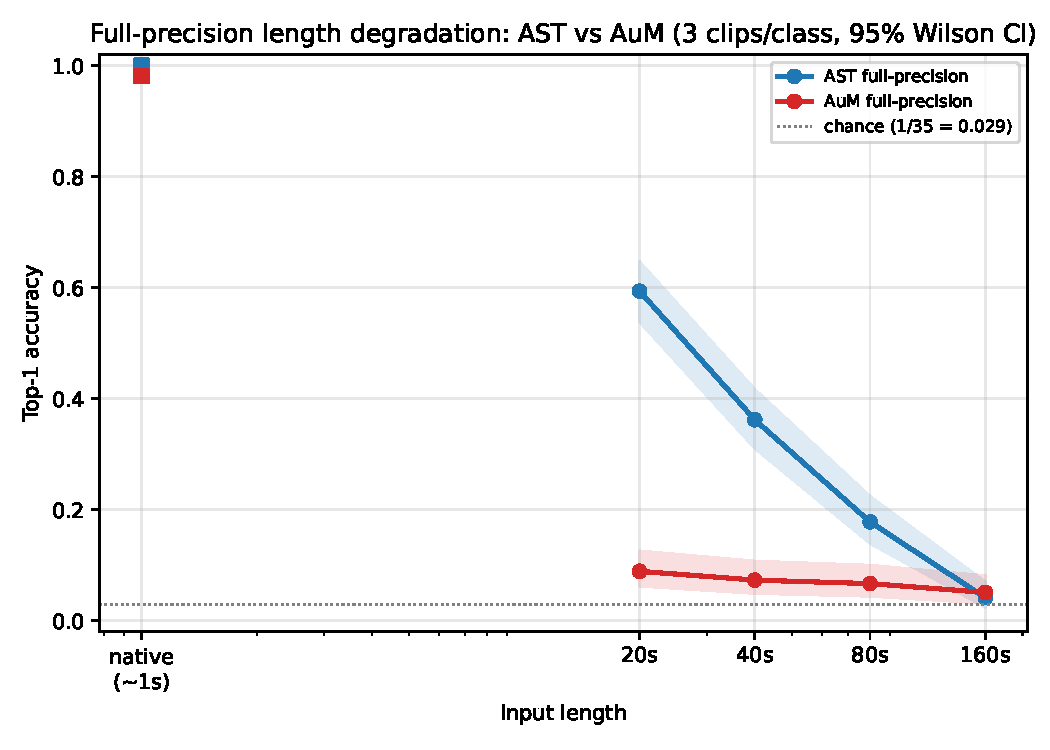
\includegraphics[width=\columnwidth]{figures/phase6_fullprecision_ast_vs_aum.pdf}
\caption{Full-precision accuracy vs.\ length. AuM collapses to near-chance immediately past training length; AST degrades gradually. Log-length slope, 20--160s: AST $-0.612$, AuM $-0.040$ -- shallower only because AuM has already hit the floor.}
\label{fig:h1}
\end{figure}

\subsection{H2: which SSM-internal tensor is fragile}
\label{sec:h2}

\begin{table}[h]
\centering
\scriptsize
\begin{tabular}{lcccc}
\toprule
Bits & $\Delta$ & $A$ & $B,C$ & state $h$ \\
\midrule
8 & .957 [.921,.986] & .971 [.943,.993] & .964 [.929,.993] & \textbf{.836} [.771,.893] \\
6 & .886 [.829,.936] & .971 [.943,.993] & .964 [.929,.993] & \textbf{.307} [.236,.386] \\
4 & \textbf{.193} [.129,.257] & .950 [.914,.986] & .964 [.929,.993] & \textbf{.079} [.036,.129] \\
\bottomrule
\end{tabular}
\caption{AuM top-1 acc., native length, $n{=}140$ (35 classes, balanced), 95\% bootstrap CI. $A,B,C$ stay within noise of full precision throughout; $h$'s 8-bit CI does not overlap $A$'s/$B,C$'s, so it is already significant at the mildest bit-width; $\Delta$'s 6- and 4-bit CIs do not overlap each other, confirming a real cliff.}
\label{tab:h2}
\end{table}

$A$ and $B,C$ are robust at every bit-width tested -- $B,C$'s accuracy is identical (96.4\%) across 8/6/4-bit. $h$ and $\Delta$ are both fragile but shaped differently (Table~\ref{tab:h2}, Figure~\ref{fig:h2}): $h$ degrades gradually, already significant at 8-bit; $\Delta$ is intact through 6-bit, then cliffs between 6- and 4-bit, landing near $h$'s own 4-bit collapse (19.3\% vs.\ 7.9\%).

\begin{figure}[h]
\centering
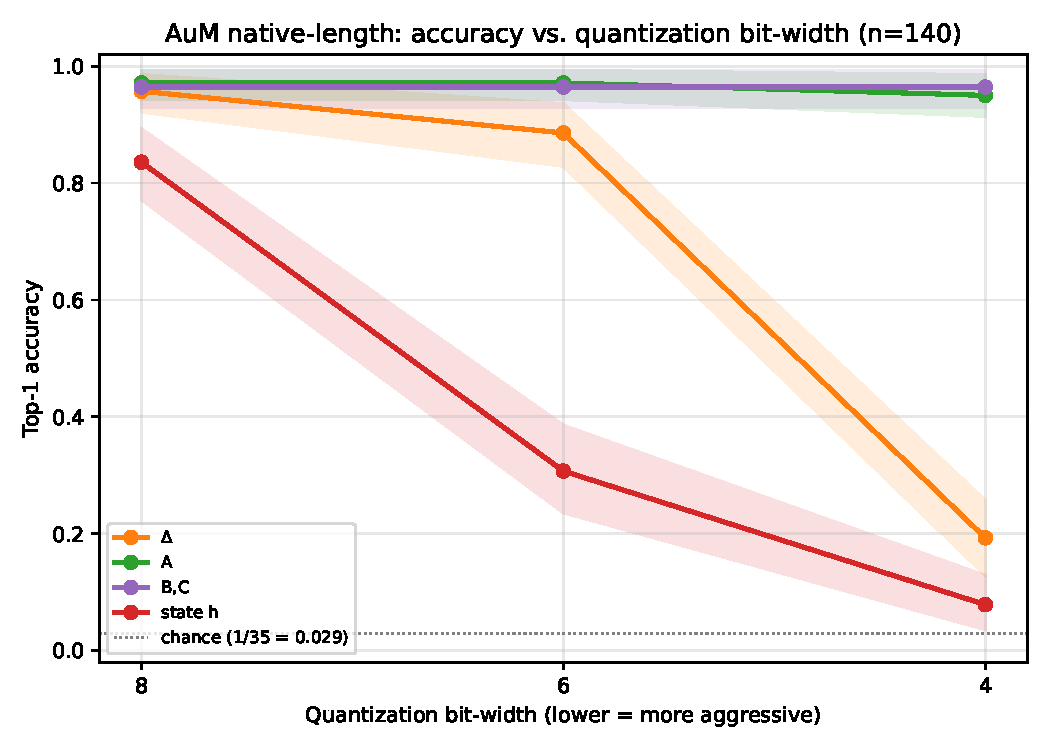
\includegraphics[width=\columnwidth]{figures/phase6_phase4_accuracy_vs_bits.pdf}
\caption{AuM native-length accuracy vs.\ SSM-internal bit-width. $A,B,C$ nearly flat; $h$ degrades from the mildest bit-width; $\Delta$ holds until a cliff between 6- and 4-bit.}
\label{fig:h2}
\end{figure}

Per-timestep divergence $\lVert h_q{-}h_{fp}\rVert_2$ ($n{=}436{,}800$ values/condition) explains the shape difference. Under state quantization, median divergence rises smoothly (0.39 $\to$ 1.13 $\to$ 2.50 at 8/6/4-bit), consistent with error accumulating every one of $\sim$65 steps once $h$ itself is corrupted. Under $\Delta$ quantization, the \emph{median} at 4-bit (0.16) is actually \emph{lower} than $A$'s/$B,C$'s own 4-bit medians (0.17, 0.26), but the \emph{mean} and \emph{max} are the largest of any condition at any bit-width (5.66, 126.8) -- most steps barely perturbed, a minority blowing up. This matches $\Delta$'s role gating $\bar{A}_t = \exp(\Delta_t A)$: a $\Delta$ error is usually harmless, but for some input-dependent values it pushes the recurrence into a regime where the error is exponentially amplified, and 4-bit pushes enough steps into that regime to break the clip.

\section{Discussion and Limitations}

This ablation uses one model pair, one dataset, and simple static per-tensor calibration -- not the rotation- or clustering-based schemes MambaQuant/Quamba2 use to work around exactly this sensitivity. The 20--160s clips are native clips spliced into background noise, not naturally long speech, so they test out-of-distribution length generalization specifically. Divergence is an absolute $L_2$ norm, not normalized by $\lVert h_{fp}\rVert$, so cross-tensor magnitudes are only loosely comparable. The H2 ablation is native-length only by design, so we do not revisit whether this fragility compounds with length the way H1's grid does; a smaller, less class-balanced earlier run suggested divergence plateaus rather than compounds within a sequence, not re-verified at this sample size.

\section{Conclusion}

For audio SSM classifiers, ``does quantization hurt the SSM more than the Transformer'' is the wrong question once length pushes the SSM past its training distribution -- it is already at chance in full precision. The right question is which part of the recurrence is load-bearing under quantization: the state $h$ and the discretization gate $\Delta$, not $A$ or $B,C$. These two fail differently -- $h$ gradually, $\Delta$ as a bit-width cliff -- a concrete target for future SSM quantization schemes, and a possible reason existing Mamba-specific PTQ recipes already single out the scan's state/activations for special treatment.

\textbf{Reproducibility.} All code, configs, calibration sets, per-clip raw results, and a full decision log (blockers, bugs, sample-size caveats included) are public.\footnote{\url{https://github.com/ayush11z/audio-ssm-quant}}

{\small
\bibliographystyle{plainnat}
\bibliography{refs}
}

\end{document}
